\section{Fase di Progettazione}
    \subsection{Struttura del Sito}
    In questa sezione presentiamo una prima bozza grafica delle varie pagine del sito. Ciò ci è servito per avere un'idea generale sull'aspetto che dovrà avere il sito e per avere una base da cui partire per lo sviluppo del layout.
    La struttura della gerarchia del sito è  suddivisa in pagine, alcune delle quali hanno delle sottopagine:
    \begin{itemize}
        \item Home;
        \item Animali:
            \begin{itemize}
                \item Tutti gli animali;
                \item Cuccioli
            \end{itemize}
        \item Eventi;
        \item Informazioni;
        \item Acquista;
        \item Area privata;
            \begin{itemize}
                \item Area amministratore/Area personale;
                \item Eventi (solo amministratore);
                \item Animali (solo amministratore);
                \item Biglietti Acquistati (solo amministratore);
                \item Eventi Prenotati (solo amministratore);
                \item Acquisti (solo amministratore);
                \item Messaggi
                \item Dati Personali (solo amministratore).
            \end{itemize}
    \end{itemize}
    \subsection{Database}
        \begin{figure}[H]
            \centering
            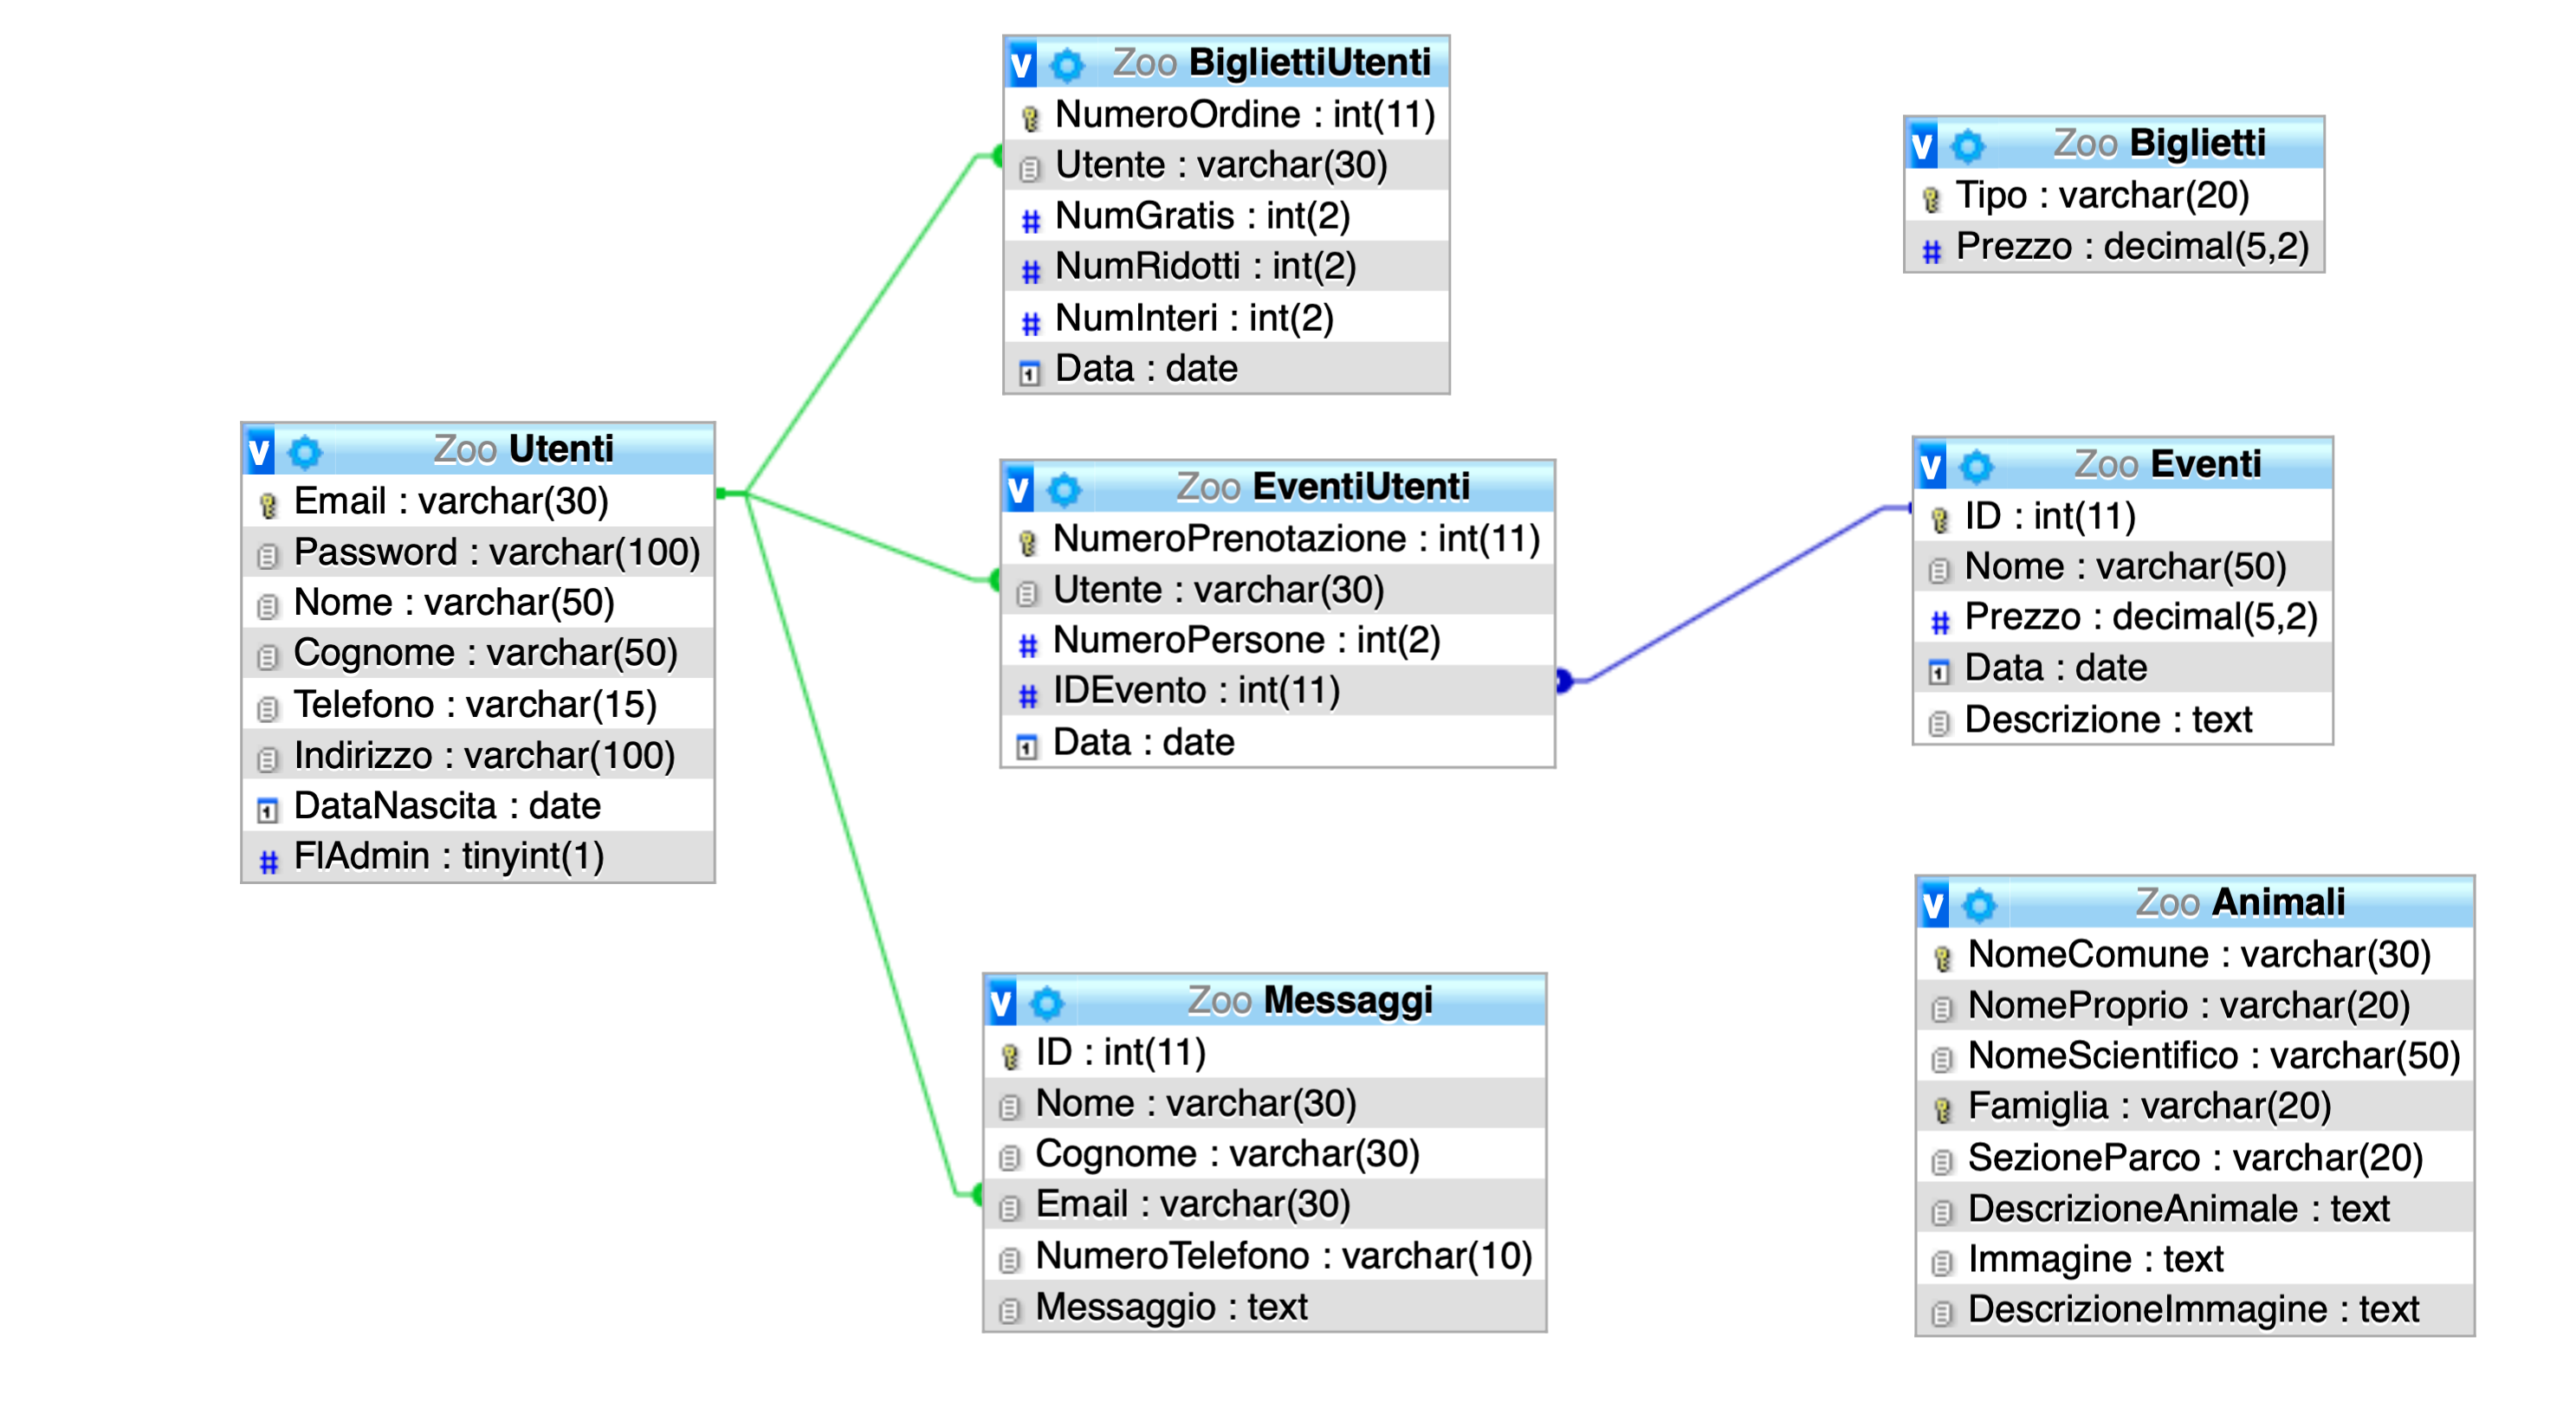
\includegraphics[width=15cm]{database.png}
            \caption{Schema del database}  \label{fig:xray}
        \end{figure}
\pagebreak